\documentclass[11pt]{article}

% ----- preamble -----
\usepackage[a4paper,margin=1.8cm]{geometry}
\usepackage{amsmath,amssymb}
\usepackage{graphicx}
\usepackage{alltt}
\usepackage{tikz}
\usepackage{tikz-cd}
\usetikzlibrary{arrows.meta,positioning,calc,fit,backgrounds,
  shapes.geometric,chains,decorations.pathreplacing}
\usepackage[most]{tcolorbox}
\usepackage{parskip}
\usepackage{xcolor}

\definecolor{ink}{RGB}{40,40,40}
\definecolor{soft}{RGB}{245,245,248}
\definecolor{grn}{RGB}{30,140,80}

% three layers + result
\definecolor{L0}{RGB}{30,90,160}     % Layer 0 : abstract scaffold (endomorphism)
\definecolor{L1}{RGB}{200,140,0}     % Layer 1 : specialization to 𝔽_{2ⁿ}
\definecolor{L2}{RGB}{150,60,160}    % Layer 2 : assembly / paper objects
\definecolor{res}{RGB}{190,50,60}    % headline result
\definecolor{inp}{RGB}{190,50,60}    % genuine arithmetic input
\definecolor{gen}{RGB}{30,90,160}    % generic / formal

\newtcolorbox{note}[1][]{colback=soft,colframe=ink,boxrule=0.4pt,
  arc=2pt,left=6pt,right=6pt,top=4pt,bottom=4pt,#1}
\newtcolorbox{leanbox}[1][]{colback=black!4,colframe=black!55,boxrule=0.4pt,
  arc=1.5pt,left=5pt,right=5pt,top=3pt,bottom=3pt,#1}

% code block: alltt keeps ^ _ % $ literal, but \( \) { } still give math/groups
\newenvironment{lean}{\begin{leanbox}\begin{alltt}\small}{\end{alltt}\end{leanbox}}

\tikzset{
  obj/.style={draw=ink,rounded corners=3pt,fill=soft,inner sep=5pt,font=\small,align=center},
  brick/.style={draw=ink,rounded corners=2pt,inner sep=6pt,font=\small,align=center,
    minimum height=13mm},
  thm/.style={draw=ink,rounded corners=3pt,fill=white,inner sep=4pt,
    font=\small,align=center,minimum height=9mm},
  arr/.style={-{Stealth[length=2.5mm]},thick},
  dep/.style={-{Stealth[length=2.4mm]},thick,ink},
}
\newcommand{\ck}{\textcolor{grn}{\checkmark}}
\newcommand{\lc}[1]{\texttt{\small #1}}
\newcommand{\phiop}{\varphi}

\title{\vspace{-1.5cm}\textbf{One endomorphism, one telescope}\\[4pt]
\large The abstract scaffold behind \texttt{DobbertinLego}: Dobbertin's Theorem~1,
step $(1)\Rightarrow(2)$}
\author{\small A picture book of the \texttt{DobbertinLego} Lean library, organized
around a single abstract gadget --- \texttt{import DobbertinLego}}
\date{}

\begin{document}
\maketitle
\vspace{-1.0cm}

\begin{note}
\textbf{The idea.} The first step of Dobbertin's Theorem~1 --- the implication
equation~(1)\,$\Rightarrow$\,equation~(2) --- rests on \emph{one} abstract object:
\begin{center}\itshape
an abelian group $A$ together with an endomorphism $\phiop : A\to A$.
\end{center}
Equivalently $A$ is a module over $\mathbb{Z}[t]$ with $t$ acting as $\phiop$; the
endomorphism lives in the ring $\mathrm{End}(A)$, where multiplication is
composition. Inside that ring are the two elements that generate everything:
\[
  \text{norm / geometric element}\quad N_m=\sum_{i<m}\phiop^i,
  \qquad\qquad
  \text{augmentation}\quad \wp=\phiop-1 .
\]
The single load-bearing algebraic fact is the \textbf{geometric telescope}
\[
  \boxed{\ \wp\circ N_m=(\phiop-1)\sum_{i<m}\phiop^{i}=\phiop^{m}-1\ }
\]
the additive shadow of the geometric series / additive Hilbert~90. It holds for
\emph{any} endomorphism of \emph{any} abelian group. Both telescoping identities
Dobbertin uses, and the fact that a trace is a bit, are specializations of it.
Every box below is a \ck\ \lc{sorry}-free Lean declaration; the headline uses only
\lc{propext}, \lc{Classical.choice}, \lc{Quot.sound}.
\end{note}

%=====================================================================
\section*{Three layers on one page}

\begin{center}
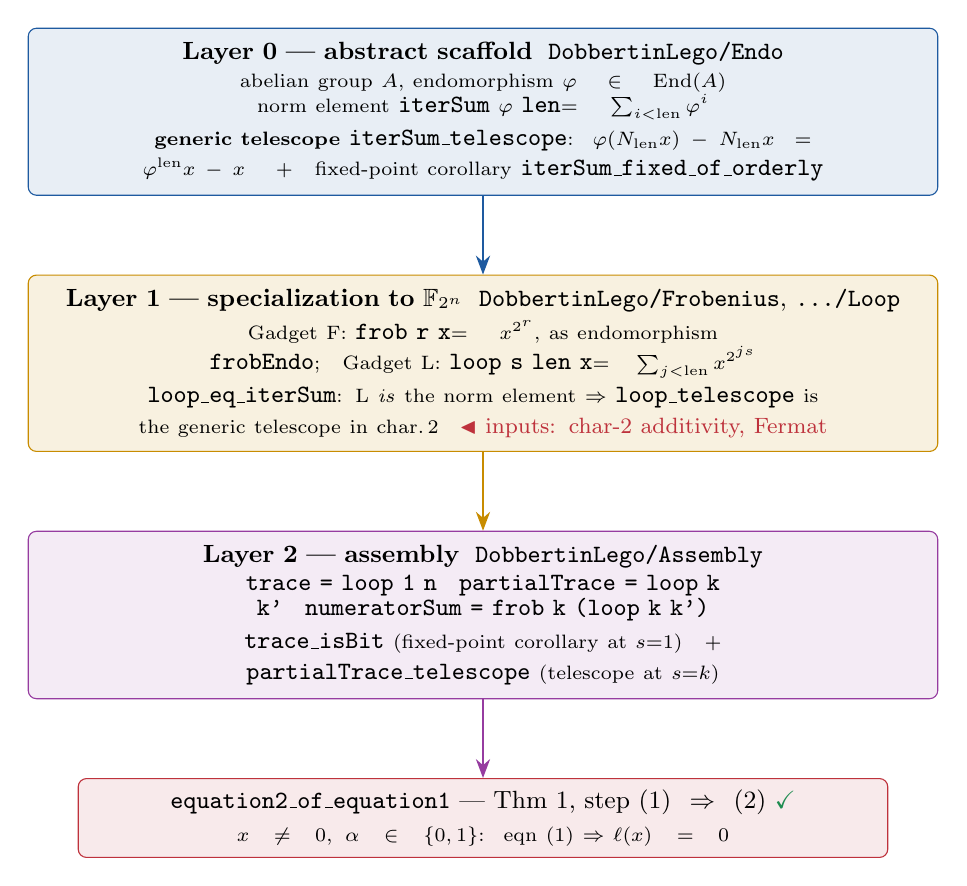
\begin{tikzpicture}[node distance=6mm]
% ---- Layer 0 : abstract scaffold ----
\node[obj,draw=L0,fill=L0!10,text width=112mm] (endo)
  {\textbf{Layer 0 --- abstract scaffold} \;\lc{DobbertinLego/Endo}\\[2pt]
   \scriptsize abelian group $A$, endomorphism $\phiop\in\mathrm{End}(A)$\qquad
   norm element \lc{iterSum }$\phiop$\lc{ len}$=\sum_{i<\text{len}}\phiop^{i}$\\[1pt]
   \scriptsize\textbf{generic telescope} \lc{iterSum\_telescope}:\;
   $\phiop(N_{\text{len}}x)-N_{\text{len}}x=\phiop^{\text{len}}x-x$
   \quad+\quad fixed-point corollary \lc{iterSum\_fixed\_of\_orderly}};

% ---- Layer 1 : specialization ----
\node[obj,draw=L1,fill=L1!12,below=10mm of endo,text width=112mm] (spec)
  {\textbf{Layer 1 --- specialization to $\mathbb{F}_{2^n}$}\;
   \lc{DobbertinLego/Frobenius}, \lc{.../Loop}\\[2pt]
   \scriptsize Gadget F: \lc{frob r x}$=x^{2^r}$, as endomorphism \lc{frobEndo};\quad
   Gadget L: \lc{loop s len x}$=\sum_{j<\text{len}}x^{2^{js}}$\\[1pt]
   \scriptsize \lc{loop\_eq\_iterSum}: L \emph{is} the norm element $\Rightarrow$
   \lc{loop\_telescope} is the generic telescope in char.\,2
   \;\;{\color{inp}\footnotesize$\blacktriangleleft$ inputs: char-2 additivity, Fermat}};

% ---- Layer 2 : assembly ----
\node[obj,draw=L2,fill=L2!10,below=10mm of spec,text width=112mm] (asm)
  {\textbf{Layer 2 --- assembly} \;\lc{DobbertinLego/Assembly}\\[2pt]
   \scriptsize \lc{trace = loop 1 n}\quad\lc{partialTrace = loop k k'}\quad
   \lc{numeratorSum = frob k (loop k k')}\\[1pt]
   \scriptsize \lc{trace\_isBit} (fixed-point corollary at $s{=}1$)\quad+\quad
   \lc{partialTrace\_telescope} (telescope at $s{=}k$)};

% ---- headline ----
\node[thm,draw=res,fill=res!10,below=10mm of asm,text width=100mm] (H)
  {\textbf{\lc{equation2\_of\_equation1}} --- Thm~1, step $(1)\Rightarrow(2)$ \ck\\[1pt]
   \scriptsize $x\neq0,\ \alpha\in\{0,1\}$:\; eqn~(1) $\Rightarrow$ $\ell(x)=0$};

\draw[dep,L0] (endo) -- (spec);
\draw[dep,L1] (spec) -- (asm);
\draw[dep,L2] (asm) -- (H);
\end{tikzpicture}
\end{center}

\noindent The arrows are literal Lean \lc{import}s. The abstract layer
\emph{organizes} the proof; the arithmetic content (characteristic~2, Fermat) is
fed in exactly once, at the Layer~0$\to$Layer~1 boundary.

%=====================================================================
\section{Layer 0 --- the abstract scaffold (\texttt{Endo.lean})}

Nothing here mentions fields, Frobenius, or characteristic. The whole layer is
about an endomorphism of an abelian group and its norm element.
\begin{lean}
variable \{A : Type*\} [AddCommGroup A]

def iterSum (\(\phiop\) : AddMonoid.End A) (len : \(\mathbb{N}\)) (x : A) : A := \(\sum\)\_\{i<len\} (\(\phiop\)^i) x

iterSum_telescope        : \(\phiop\)(iterSum \(\phiop\) len x) - iterSum \(\phiop\) len x
                             = (\(\phiop\)^len) x - x                       \ck  -- additive Hilbert 90
iterSum_fixed_of_orderly : \(\phiop\)^n = 1 \(\Rightarrow\)
                             \(\phiop\)(iterSum \(\phiop\) n x) = iterSum \(\phiop\) n x   \ck  -- norm lands in fixed points
\end{lean}
\emph{The telescope}, in one line: applying one more $\phiop$ to $N_{\text{len}}$
and subtracting $N_{\text{len}}$ cancels every interior iterate $\phiop^1,\dots,
\phiop^{\text{len}-1}$, leaving the endpoints $\phiop^{\text{len}}-1$. The
\emph{fixed-point corollary} is the same identity when $\phiop$ has finite order
($\phiop^n=1$, so $\phiop^n-1=0$): the full norm element is $\phiop$-invariant,
i.e. it lands in the fixed subgroup.

\begin{center}
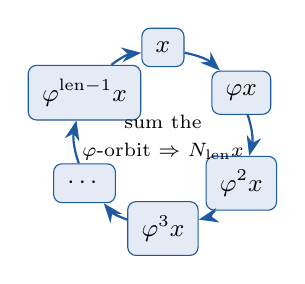
\begin{tikzpicture}[scale=1,every node/.style={font=\small}]
\def\R{1.15}
\foreach \a/\lab in {90/x,30/\phiop x,-30/\phiop^2 x,-90/\phiop^3 x,
    -150/\cdots,150/\phiop^{\text{len}-1}x}{
  \node[obj,draw=L0,fill=L0!12] (n\a) at (\a:\R) {$\lab$};}
\foreach \a/\b in {90/30,30/-30,-30/-90,-90/-150,-150/150,150/90}{
  \draw[arr,L0] (n\a) to[bend left=16] (n\b);}
\node[align=center] at (0,0) {\scriptsize sum the\\[-1pt]\scriptsize $\phiop$-orbit
  $\Rightarrow$ $N_{\text{len}}x$};
\end{tikzpicture}
\end{center}

%=====================================================================
\section{What is a genuine input, and what is formal}

The value of the abstract layer is that it makes visible \emph{which} facts are
generic module theory and \emph{which} are irreducible arithmetic inputs of the
finite field. The three ``load-bearing'' facts split cleanly:

\begin{center}\small
\renewcommand{\arraystretch}{1.35}
\begin{tabular}{@{}p{4.4cm} p{5.1cm} p{5.6cm}@{}}
\textbf{fact} & \textbf{abstract home} & \textbf{status}\\ \hline
Freshman's dream $(a{+}b)^2=a^2{+}b^2$
  & $\phiop$ is an \emph{additive} endomorphism (lives in $\mathrm{End}(A)$)
  & {\color{inp}\textbf{genuine char-2 input}} --- Mathlib \lc{frobenius}, \lc{add\_pow\_char\_pow}\\
Telescoping $S^{2^k}{+}S=x^2{+}x$
  & $(\phiop{-}1)\sum\phiop^i=\phiop^m{-}1$
  & {\color{gen}\textbf{formal}} --- pure module theory (\lc{iterSum\_telescope})\\
$\mathrm{Tr}(x)\in\{0,1\}$
  & norm element lands in fixed subgroup ($\phiop^n{=}1$)
  & {\color{gen}formal skeleton} (\lc{iterSum\_fixed\_of\_orderly}) + {\color{inp}input} $\mathbb{F}_2=\{0,1\}$\\
$\phiop^n=\mathrm{id}$ (Fermat)
  & $\phiop$ has finite order $n$ (cyclic Galois group)
  & {\color{inp}\textbf{finite-field input}} --- Mathlib \lc{FiniteField.pow\_card}\\
$k'k\equiv1$ collapses $\phiop^{k'k}$ to $\phiop$
  & multiplication in $\mathbb{Z}/n=\mathrm{ord}(\phiop)$
  & {\color{gen}formal} --- periodicity \lc{frob\_periodic}\\
\end{tabular}
\end{center}

\noindent In one sentence: category/module theory supplies the \emph{shape} (the
telescope on a dualizable / finite-order object); characteristic~2 supplies only
two atoms --- $\phiop$ is additive, and the fixed subgroup is the two-element field.

%=====================================================================
\section{Layer 1 --- specialization to $\mathbb{F}_{2^n}$ (\texttt{Frobenius}, \texttt{Loop})}

The bridge is short: the Frobenius $x\mapsto x^{2^{s}}$ is additive
(\lc{frob\_add}), so it \emph{is} an element \lc{frobEndo s} of $\mathrm{End}(F)$,
its iterates are its ring powers, and Fermat is finite order.
\begin{lean}
def frob (r : \(\mathbb{N}\)) (x : F) : F := x ^ (2 ^ r)                         -- Gadget F
def frobEndo (s : \(\mathbb{N}\)) : AddMonoid.End F := AddMonoidHom.mk' (frob s) (frob_add s)

frobEndo_pow_apply : (frobEndo s ^ j) x = frob (j*s) x            \ck  -- iterates = ring powers
frobEndo_pow_card  : |F|=2^n \(\Rightarrow\) frobEndo n = 1                    \ck  -- Fermat = finite order

def loop (s len : \(\mathbb{N}\)) (x : F) : F := \(\sum\)\_\{j<len\} frob (j*s) x            -- Gadget L
loop_eq_iterSum : loop s len x = iterSum (frobEndo s) len x       \ck  -- L IS the norm element

loop_telescope  : frob s (loop s len x) + loop s len x
                    = frob (len*s) x + x                          \ck  -- generic telescope, char 2
\end{lean}
Because \lc{loop} \emph{is} the abstract norm element, \lc{loop\_telescope} is no
longer a bespoke induction: it is \lc{iterSum\_telescope} read in
characteristic~2, where $-1=+1$ turns the subtraction into addition.

%=====================================================================
\section{Layer 2 --- assembly, and the headline}

The paper's three objects are one settings of the \emph{same} norm element, and
its two auxiliary facts are two specializations of the \emph{same} scaffold.
\begin{center}\small
\renewcommand{\arraystretch}{1.3}
\begin{tabular}{@{}l l l@{}}
\textbf{paper object} & \textbf{abstract element} & \textbf{Lean}\\ \hline
trace $\mathrm{Tr}(x)$ & $N_n$ at $\phiop=$Frob$^1$ & \lc{trace n x = loop 1 n x}\\
partial trace $P(x)$ & $N_{k'}$ at $\phiop=$Frob$^k$ & \lc{partialTrace k k' x = loop k k' x}\\
numerator sum $S(x)$ & $\phiop^k N_{k'}$ & \lc{numeratorSum k k' x = frob k (loop k k' x)}\\ \hline
$\mathrm{Tr}(x)\in\{0,1\}$ & fixed-point corollary & \lc{trace\_isBit}\\
$S+P=x^2+x$ & telescope at $s{=}k$ & \lc{partialTrace\_telescope}\\
\end{tabular}
\end{center}
\begin{lean}
theorem equation2_of_equation1 (hn : |F| = 2^n) (hkk' : k*k' % n = 1)
    (h\(\alpha\) : \(\alpha\)=0 \(\vee\) \(\alpha\)=1) (hx : x \(\neq\) 0) (h : equation1 n k k' \(\alpha\) c x) :
    linearized k c x = 0                                              \ck
\end{lean}
The proof collapses $\alpha\cdot\mathrm{Tr}(x)$ to a bit (via \lc{trace\_isBit}),
solves (1) for $P$ using $S=P^{2^k}$ and $S+P=x^2+x$, raises to the $2^k$ power
(Frobenius additive), and divides by $x^{2^k}\neq0$ to read off $\ell(x)=0$.
\emph{Why $x\neq0$:} at $x=0$ the cleared (1) holds vacuously while
$\ell(0)=1\neq0$.

%=====================================================================
\section*{Compositional build diagram}

\begin{center}
{\footnotesize
\begin{tikzcd}[column sep=0.75cm,row sep=0.9cm]
|[draw=L0,rounded corners,fill=L0!8]| \text{\lc{iterSum}}
  \arrow[d,"\text{induction}"']
  &&\\
|[draw=L0,rounded corners,fill=L0!8]| \text{\lc{iterSum\_telescope}}
  \arrow[r,"\phiop=\text{frobEndo}"]
  \arrow[d,"\phiop^n=1"']
  & |[draw=L1,rounded corners,fill=L1!12]| \text{\lc{loop\_telescope}}
  \arrow[r,"s=k"]
  & |[draw=L2,rounded corners,fill=L2!10]| \text{\lc{partialTrace\_telescope}}
  \arrow[dr]\\
|[draw=L0,rounded corners,fill=L0!8]| \text{\lc{iterSum\_fixed\_of\_orderly}}
  \arrow[r,"s=1"']
  & |[draw=L2,rounded corners,fill=L2!10]| \text{\lc{trace\_isBit}}
  \arrow[rr]
  && |[draw=res,rounded corners,fill=res!10]| \text{\lc{equation2\_of\_equation1}}
\end{tikzcd}
}
\end{center}

\begin{note}
\textbf{One sentence.} Step $(1)\Rightarrow(2)$ of Dobbertin's Theorem~1 is
\emph{one} abstract gadget --- an abelian group with an endomorphism, its norm
element, and the single geometric telescope $(\phiop{-}1)\sum\phiop^i=\phiop^m{-}1$
--- specialized to the Frobenius of $\mathbb{F}_{2^n}$; the paper's trace, partial
trace and numerator sum are that norm element at three settings, its two auxiliary
facts are the telescope and its finite-order corollary, and the arithmetic of
characteristic~2 enters only as the two irreducible atoms (additivity, two-element
fixed field). \emph{Scope:} the first step only; Theorem~1 proper and the
difference-set half are not part of this minimal library.
\end{note}

\bigskip
\begin{center}\scriptsize
Source: \lc{DobbertinLego/} (\lc{Endo}, \lc{Frobenius}, \lc{Loop}, \lc{Assembly})
and \lc{DobbertinLego.lean}. Paper: H.~Dobbertin, \emph{Kasami Power Functions,
Permutation Polynomials and Cyclic Difference Sets} (1999), proof of Theorem~1,
step (1)\,$\Rightarrow$\,(2).
\end{center}

\end{document}
